\documentclass[11pt]{article}

\usepackage{booktabs}
\usepackage{dcolumn} 
\usepackage{epstopdf}
\usepackage{fourier}
\usepackage{fullpage}
\usepackage{graphicx}
\usepackage{hyperref}
\usepackage{longtable} 
\usepackage{natbib}
\usepackage{rotating}
\usepackage{tabularx}
\usepackage{amsmath}
% \usepackage{algorithmic} 
% \usepackage{algorithm2e}

\hypersetup{
  colorlinks = TRUE,
  citecolor=blue,
  linkcolor=red,
  urlcolor=black
}

\begin{document} 

\title{What determines (perceived) wages?}

\date{\today}

\author{ John J. Horton \\ NYU Stern \footnote{ Author contact information, datasets and code are currently or will be available at \href{http://www.john-joseph-horton.com/}{http://www.john-joseph-horton.com/}. } }
\maketitle

\begin{abstract}
\noindent  Here is a really great abstract.  \newline
\noindent JEL J01, J24, J3
\end{abstract} 

\section{Introduction}
\section{Conceptual Framework} 

Would-be labor force participants need knowledge about what various occupations pay--and will pay in the future---to plan their careers and make wise human capital decisions. 

Numerous studies have documented that simply providing information can have strong effects on behavior (for example, \cite{jensen2010perceived} for the returns to education and \cite{dupas2009teenagers} to the benefits of changed sexual behavior).  


These kinds of information interventions are predictated on some kind
of incomplete information that can be remedied. 


This was the justification for including the Knowledge of the World of Work (KWW) test in the NLSY. 
The original KWW consisted of matching job descriptions to job titles and a section of relative comparisons of wages. 
The KWW was predictive of positive future economic success and was correlated with higher wages, greater tenure etc \citep{kohen1975133}. 
It is unclear whether KWW was just measuring intelligence of ability---KWW is sometimes used as an instrument for IQ to deal with measurement error. 


This study does a number of things. 
It examines the correlates of 

Presumably would-be labor market participants learn about wages from media sources, friends and family and, perhaps, official government statistics. 

Corrective informational interventions 

Perhaps more knowledgeable 

Identifying deficiencies 

\cite{jensen2010perceived} 

The short time taken to answer questions suggests that workers are not doing research. 

The wisdom of crowds hypotheses suggests that combining 

Estimates of the mean hourly wages for a selection of BLS occupations by workers on Mechanical Turk explains over 70\% of the variation in wages according to the OES (Occupational Employment Statistics).  

Error rates are decreasing the total employment in that occupation. 
The more people workers know with that occupation, the more 

\cite{snowberg2011prediction}
\cite{kohen1975} 
\cite{dupas2009teenagers} 

-Test whether social knowledge is mediated by the total employment 
-Correct perception errors 
-Test whether workers are clustered in their wage perceptions

For each of the top 99 BLS occupations---as measured by total occupation---I asked workers on Mechanical Turk several questions: 
\begin{itemize}
\item Did they know approximately what this job consists of? 
\item How many people did they know with that job? 
\item What was their estimate of the hourly wage for that job 
\item What was their estimate of wages for this job in the future.
\item What was their estimate of the future employer for this job. 
\end{itemize} 


How important is it to know someone who has this job? 
Do various correlations exist in this population? 

It is not difficult to assess this knowledge. 

\cite{smith1999wealth} had some great ideas! 

\section{Results}

\begin{figure}
\caption{Knowledge by occupation title} 
\centering
\begin{minipage}{0.85 \linewidth}
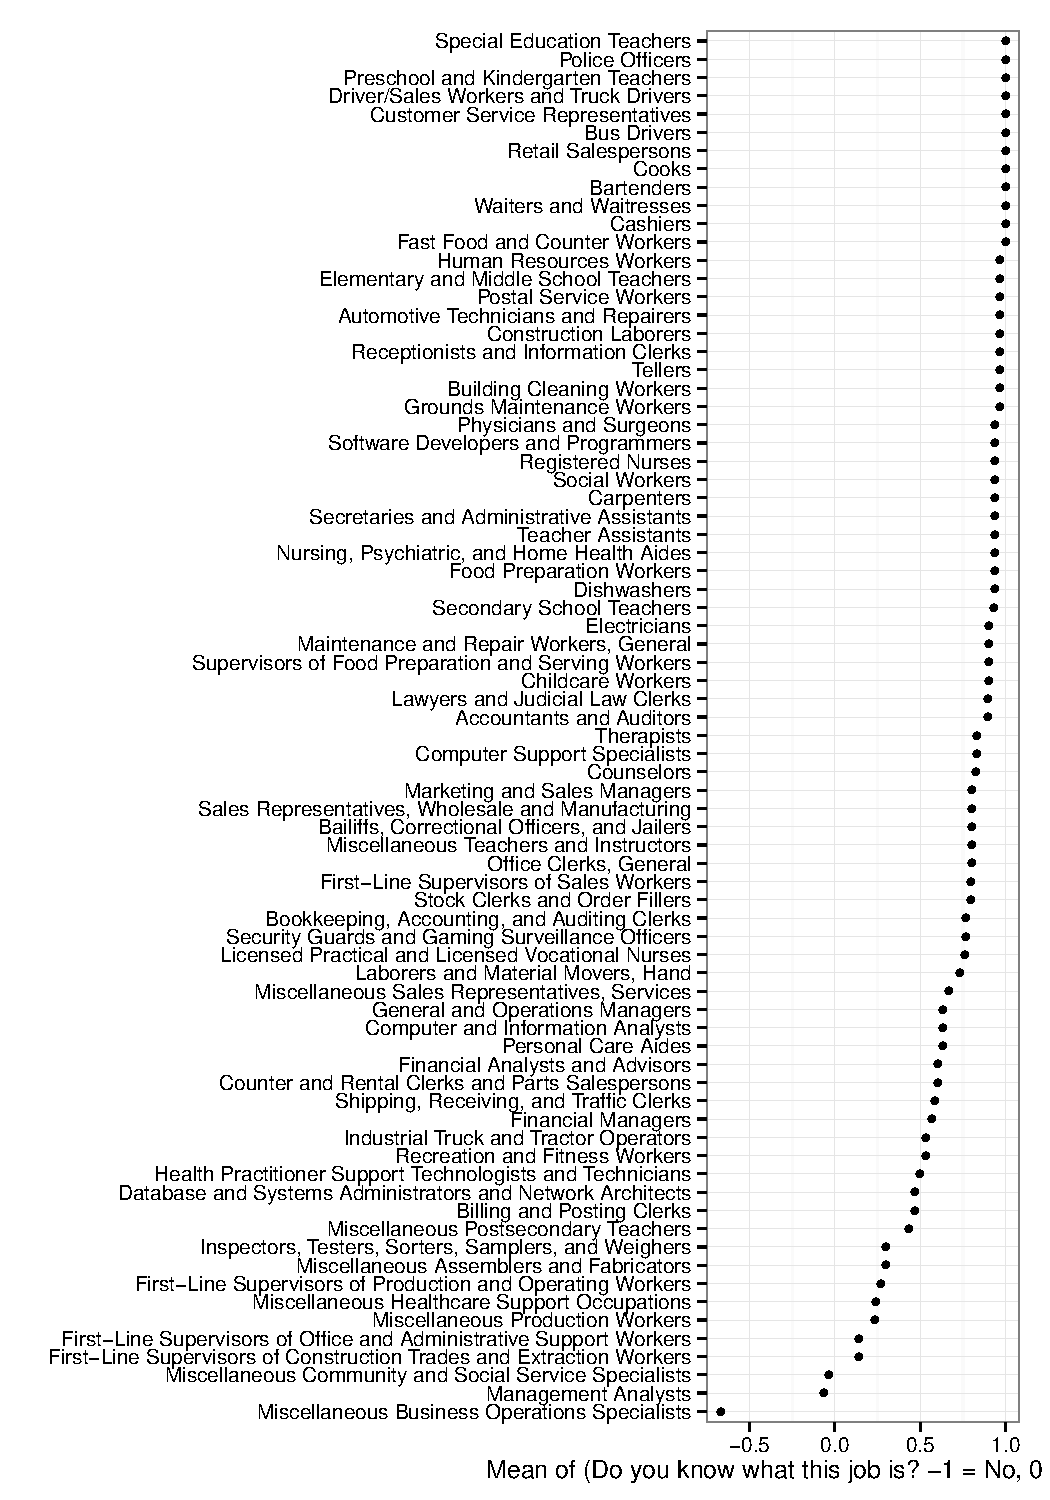
\includegraphics[width = \linewidth]{./plots/knowledge_by_occupation.pdf}
\end{minipage}  
\end{figure} 

\begin{figure}
\caption{Wage and self-reported knowledge of what job consists of} 
\centering
\begin{minipage}{0.85 \linewidth}
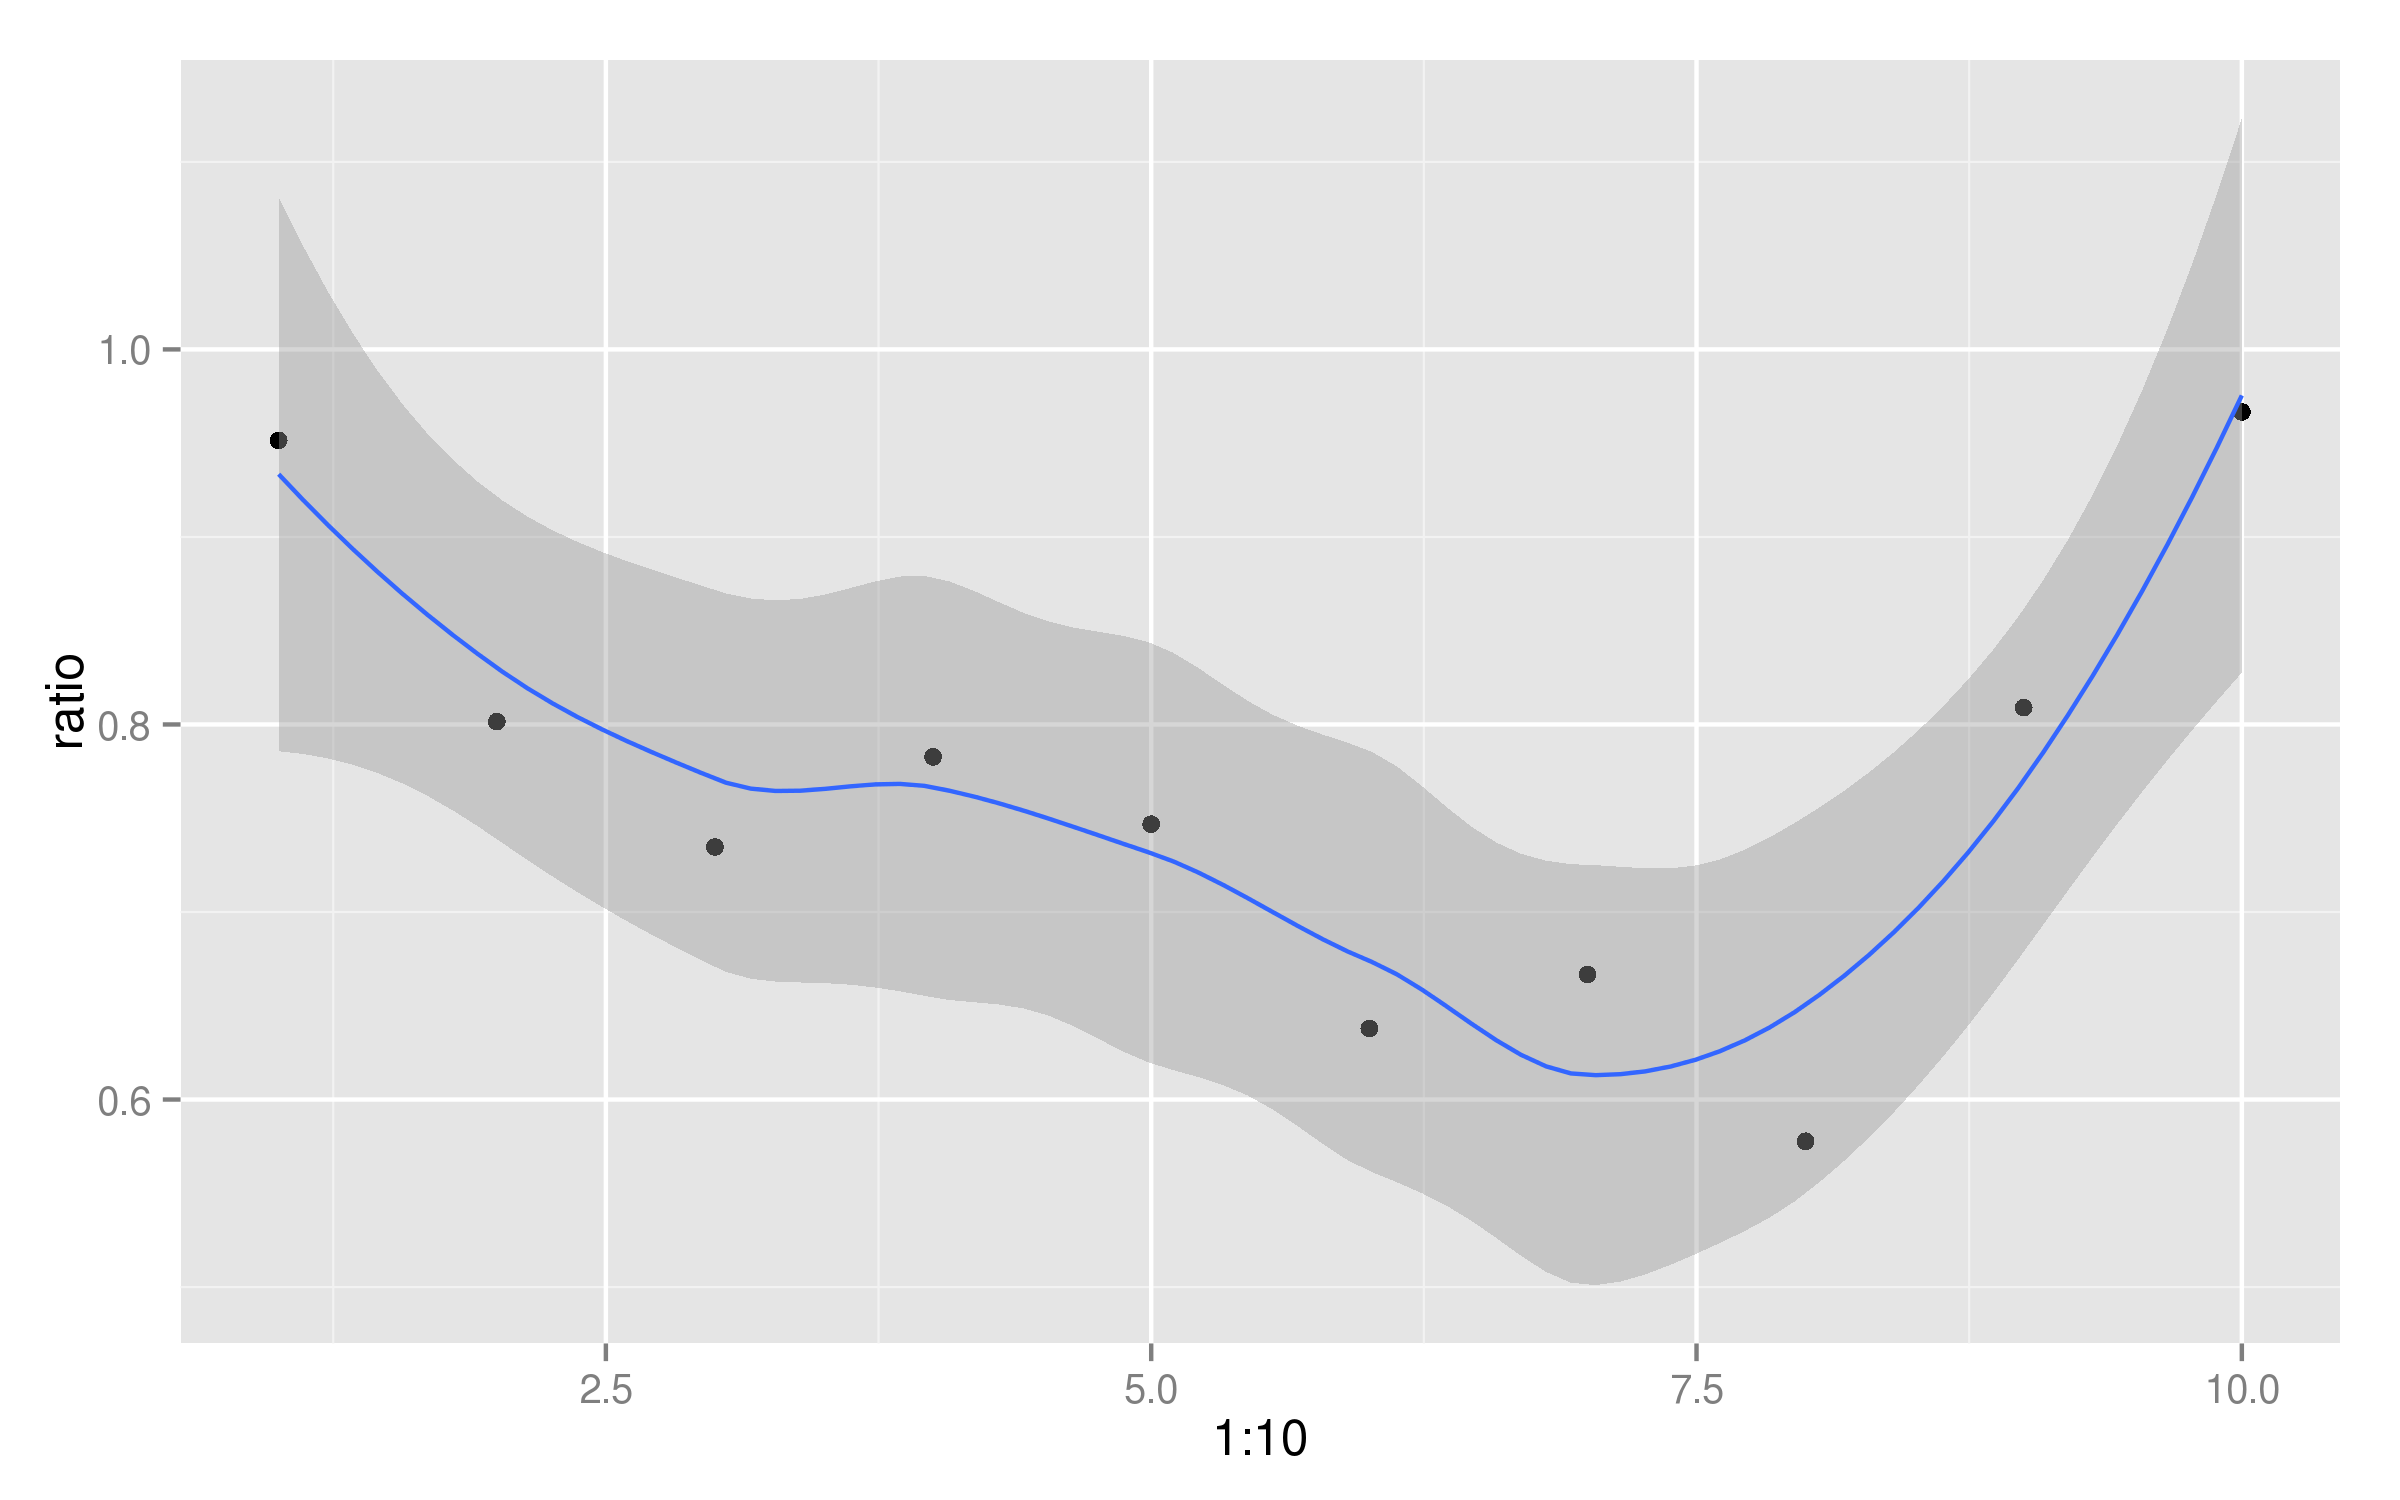
\includegraphics[width = \linewidth]{./plots/knowledge_wage.png}
\end{minipage}  
\end{figure} 


\begin{figure}
\caption{Wage trends} 
\centering
\begin{minipage}{0.85 \linewidth}
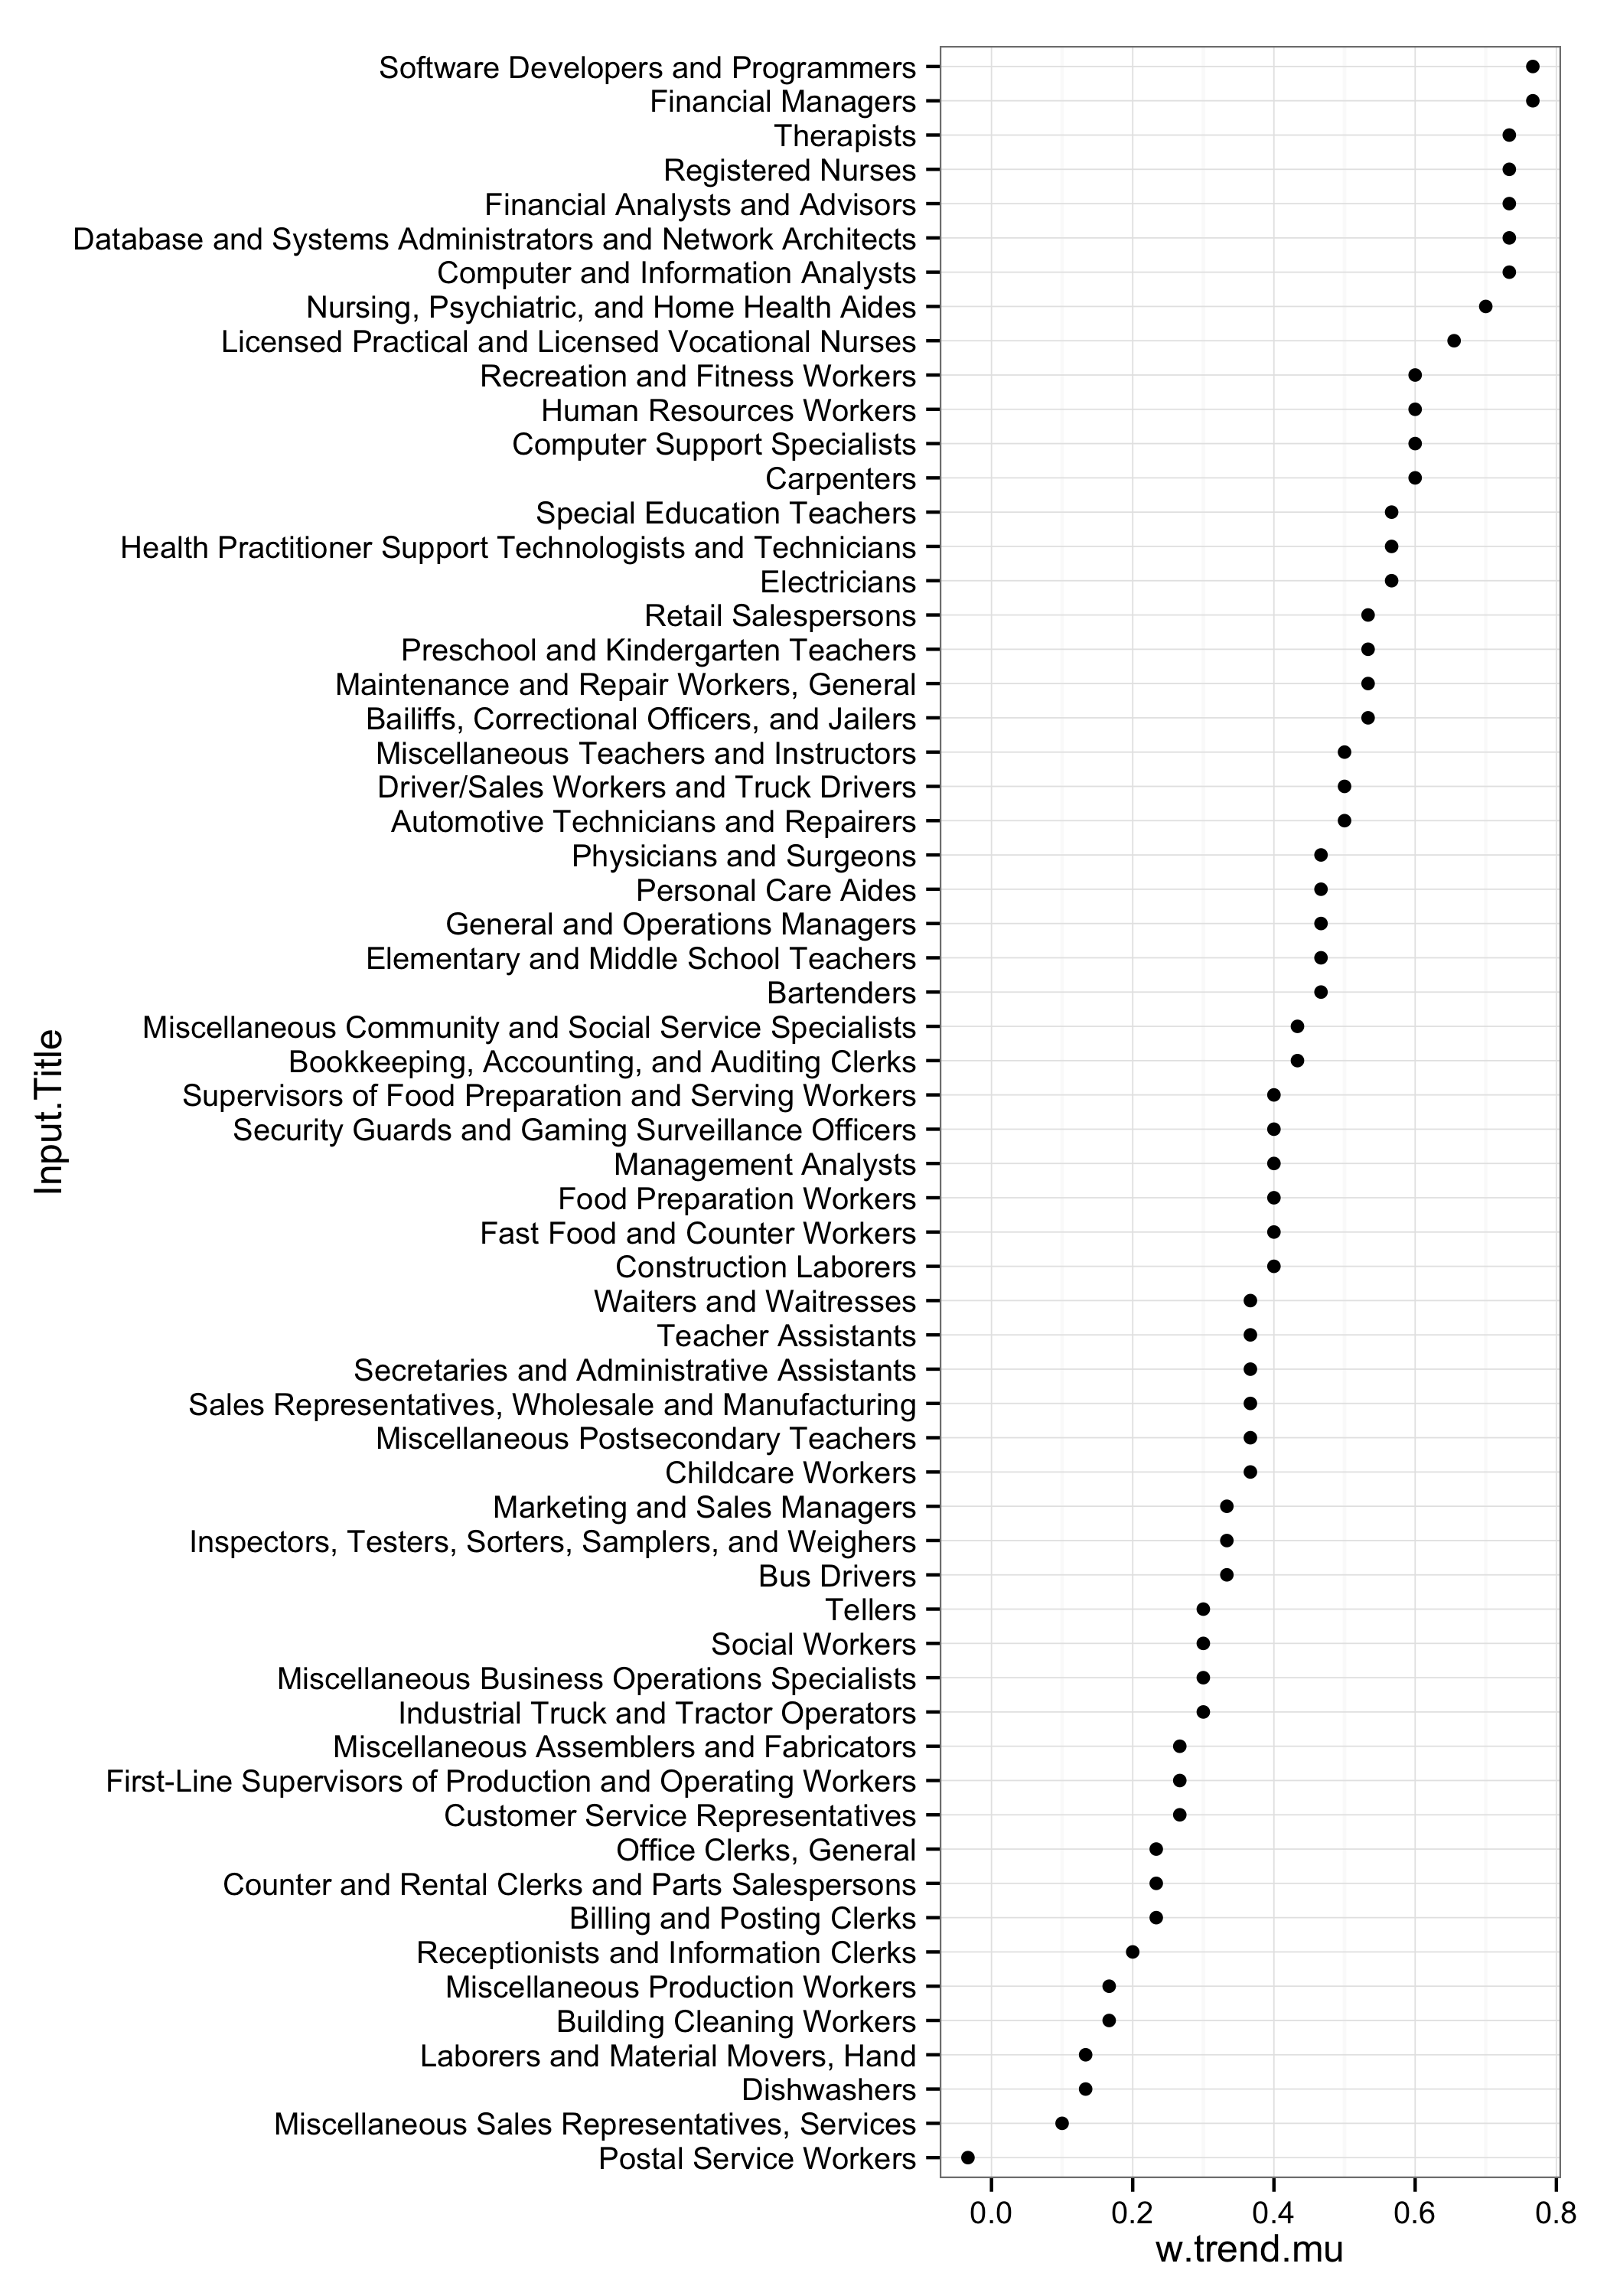
\includegraphics[width = \linewidth]{./plots/wage_trends.png}
\end{minipage}  
\end{figure} 


\begin{figure}
\caption{Knowledge by total employment} 
\centering
\begin{minipage}{0.85 \linewidth}
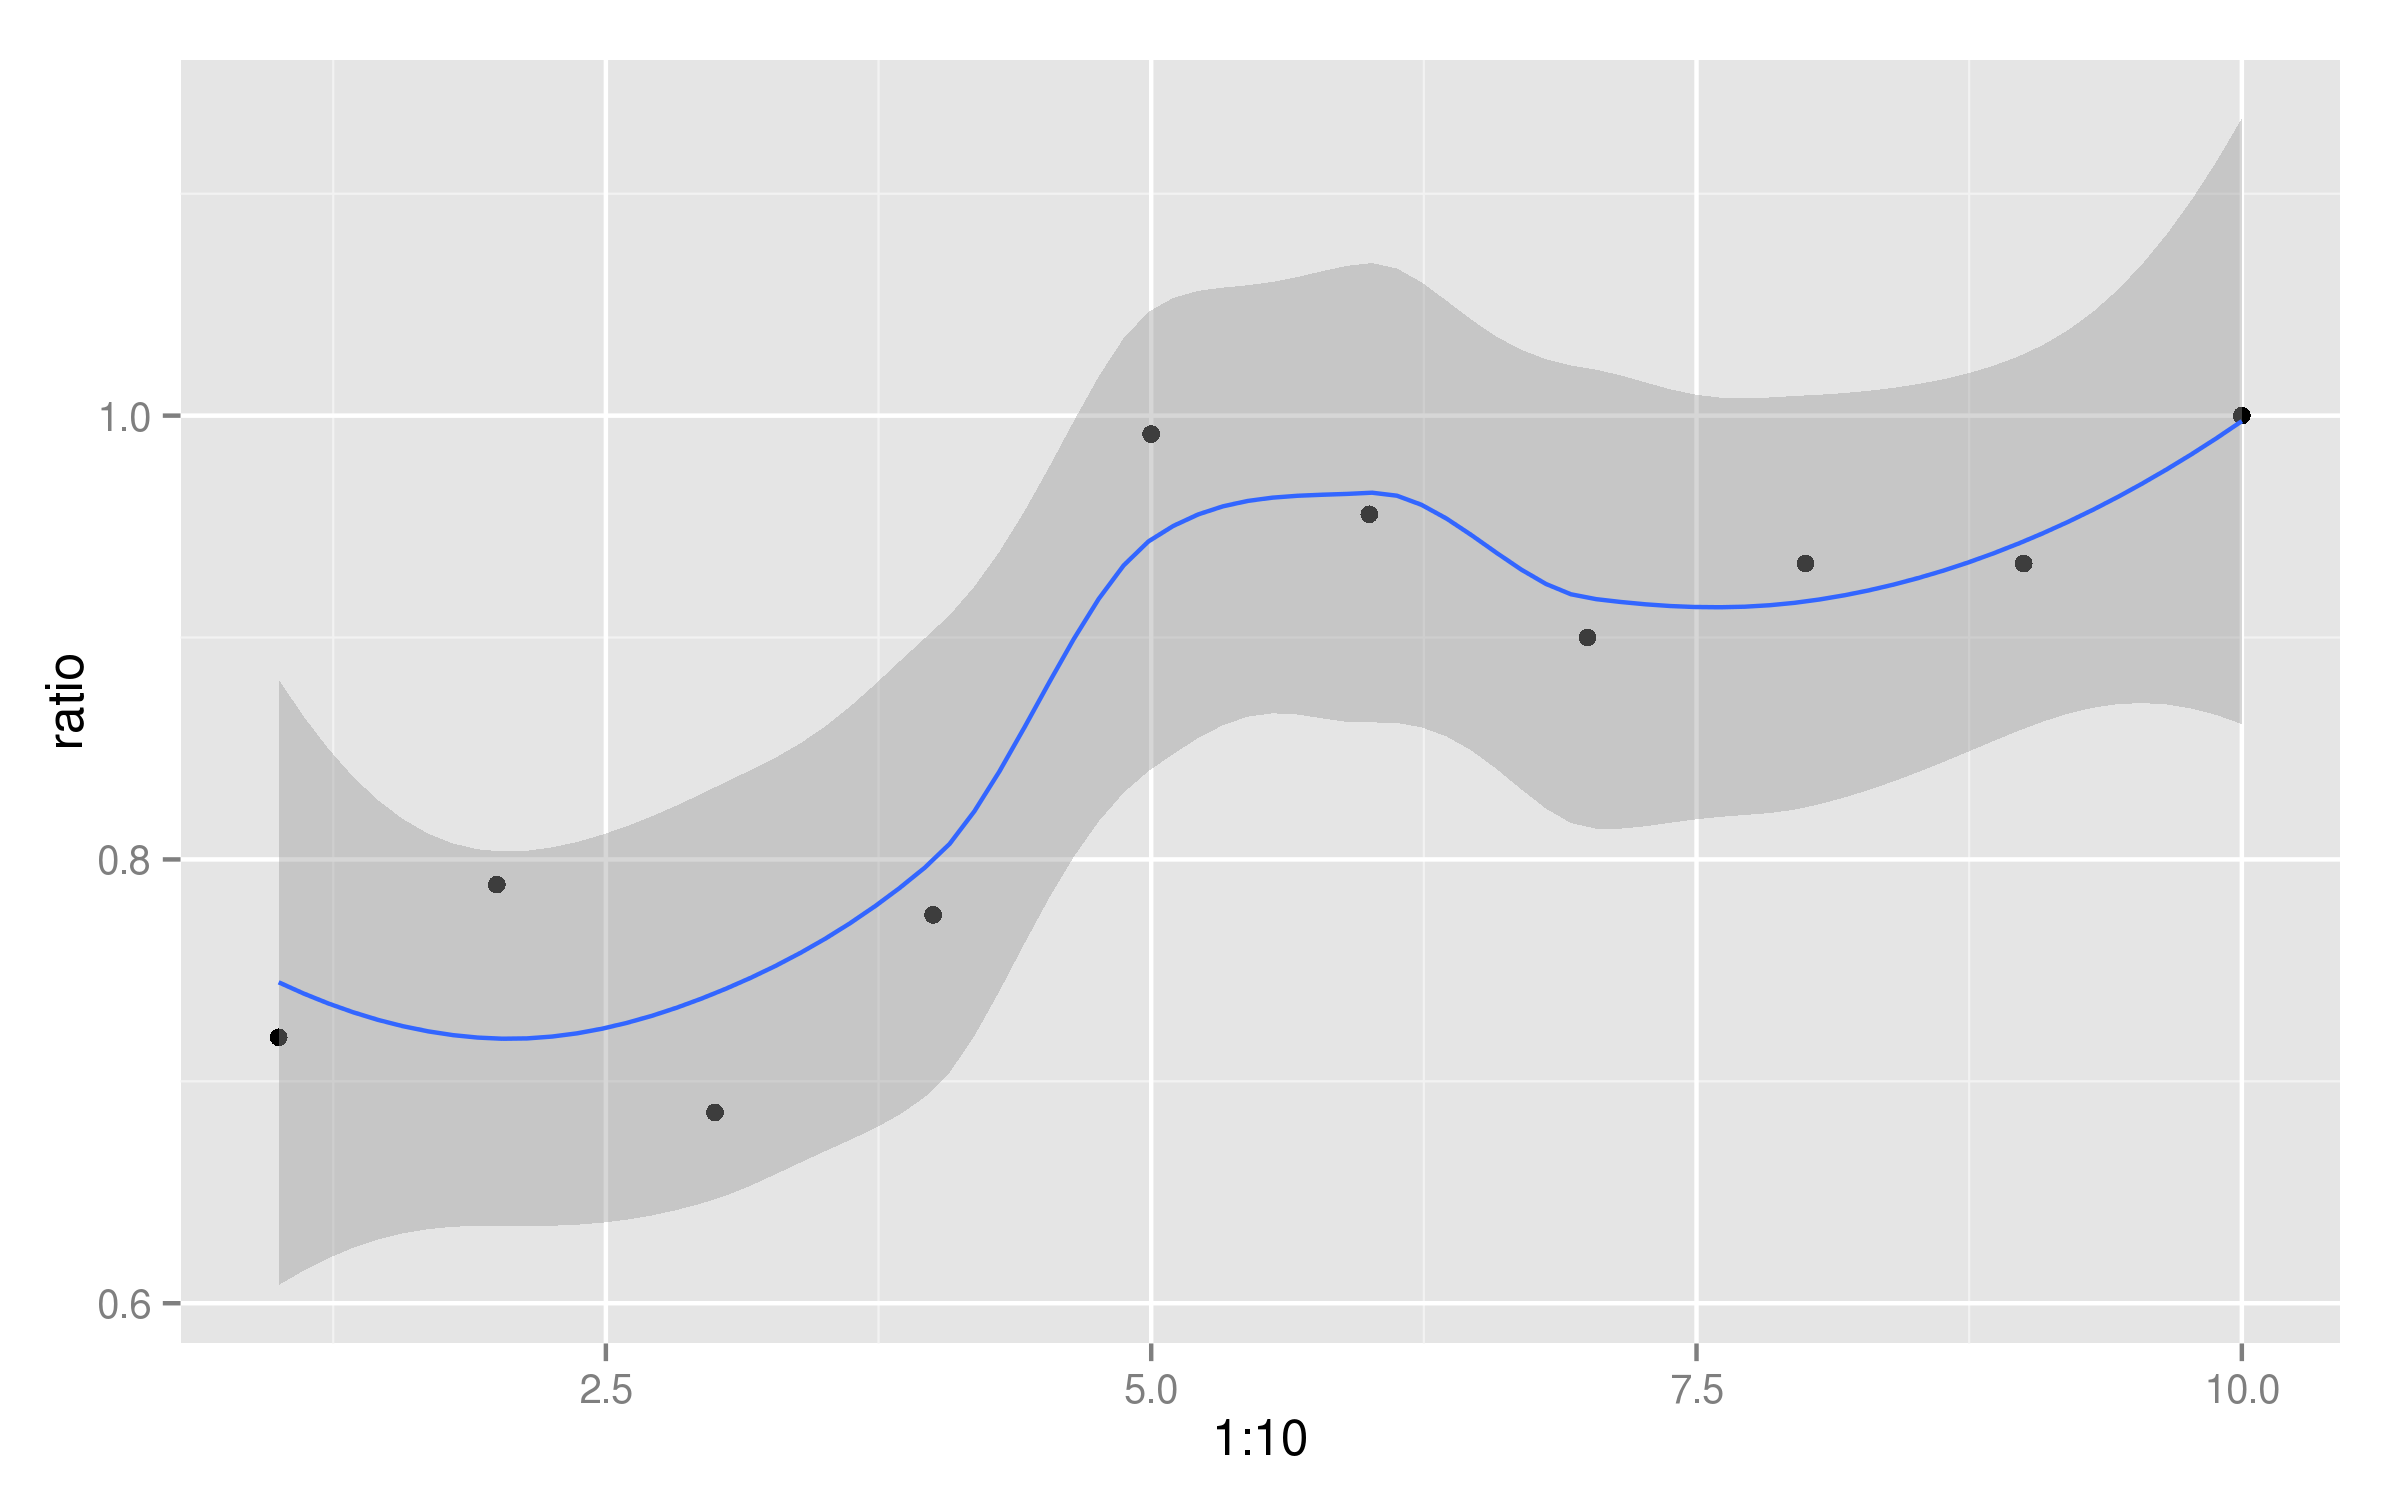
\includegraphics[width = \linewidth]{./plots/knowledge_emp.png}
\end{minipage}  
\end{figure} 


% latex table generated in R 3.0.2 by xtable 1.7-1 package
% Tue Nov 12 04:22:34 2013
\begin{table}[ht]
\centering
\begin{tabular}{rll}
  \hline
 &      OES &      MTSO \\ 
  \hline
1 & Min.   :0.0000   & Min.   :18.05   \\ 
  2 & 1st Qu.:0.5000   & 1st Qu.:28.54   \\ 
  3 & Median :0.7000   & Median :32.14   \\ 
  4 & Mean   :0.7152   & Mean   :34.29   \\ 
  5 & 3rd Qu.:0.9000   & 3rd Qu.:39.77   \\ 
  6 & Max.   :1.4000   & Max.   :60.57   \\ 
   \hline
\end{tabular}
\caption{RSE for Hourly Wages in OES and MTSO datasets (all obs.)} 
\label{tab:rse_oes_mtso1}
\end{table}


% latex table generated in R 3.0.2 by xtable 1.7-1 package
% Tue Nov 12 04:22:47 2013
\begin{table}[ht]
\centering
\begin{tabular}{rll}
  \hline
 &      OES &      MTSO \\ 
  \hline
1 & Min.   :0.0000   & Min.   :15.01   \\ 
  2 & 1st Qu.:0.5000   & 1st Qu.:25.82   \\ 
  3 & Median :0.7000   & Median :30.96   \\ 
  4 & Mean   :0.7173   & Mean   :32.69   \\ 
  5 & 3rd Qu.:0.9000   & 3rd Qu.:40.00   \\ 
  6 & Max.   :1.4000   & Max.   :65.93   \\ 
  7 &  & NA's   :2   \\ 
   \hline
\end{tabular}
\caption{RSE for Hourly Wages in OES and MTSO datasets (filtered)} 
\label{tab:rse_oes_mtso2}
\end{table}


\begin{tiny} 
%%%%%%%%%%%%%%%%%%%%%%%%%%%%%%%%%%%%%%%%%%%%%%%%%%%%%%%%%%%%%%%%%%%%%%%%%%%%%%%%%%%%%%%%%%%%%%%%%%%%%%%%%%%%%%%%%%%%%%%%%%%%%
%
% Calls:
% 1:  glm(formula = error ~ know * social + log(TOT_EMP) + H_WAGE, data = mturk.df) 
% 2:  glm(formula = error ~ know * social + H_WAGE, data = mturk.df) 
% 3:  glm(formula = error ~ social + H_WAGE + log(TOT_EMP), data = mturk.df) 
% 4:  lmer(formula = error ~ know * social + log(TOT_EMP) + H_WAGE + (1 | Input.Title), data = mturk.df) 
% 5:  glm(formula = error ~ know * social + log(TOT_EMP) + H_WAGE + I(log(Answer.wage) > 3), data = mturk.df) 
%
%%%%%%%%%%%%%%%%%%%%%%%%%%%%%%%%%%%%%%%%%%%%%%%%%%%%%%%%%%%%%%%%%%%%%%%%%%%%%%%%%%%%%%%%%%%%%%%%%%%%%%%%%%%%%%%%%%%%%%%%%%%%%
\begin{tabular}{lcD{.}{.}{7}cD{.}{.}{7}cD{.}{.}{7}cD{.}{.}{7}cD{.}{.}{7}}
\toprule
&&\multicolumn{1}{c}{1} && \multicolumn{1}{c}{2} && \multicolumn{1}{c}{3} && \multicolumn{1}{c}{4} && \multicolumn{1}{c}{5}\\
\midrule
(Intercept)                  &  &  -0.058      &&  0.137^{***} &&   0.004      &&  -0.025      &&   0.034     \\
                             &  &  (0.121)     &&  (0.038)     &&  (0.117)     &&  (0.274)     &&  (0.116)    \\
know                         &  &   0.043      &&   0.046      &&              &&   0.035      &&   0.048     \\
                             &  &  (0.038)     &&  (0.038)     &&              &&  (0.035)     &&  (0.036)    \\
social                       &  & -0.042^{*}   && -0.041^{*}   && -0.013^{*}   &&  -0.033      && -0.037^{*}  \\
                             &  &  (0.019)     &&  (0.019)     &&  (0.006)     &&  (0.018)     &&  (0.018)    \\
log(TOT_EMP)                 &  &   0.014      &&              &&   0.013      &&   0.012      &&   0.007     \\
                             &  &  (0.008)     &&              &&  (0.008)     &&  (0.020)     &&  (0.008)    \\
H_WAGE                       &  &  0.008^{***} &&  0.007^{***} &&  0.008^{***} &&  0.008^{***} &&  0.010^{***}\\
                             &  &  (0.000)     &&  (0.000)     &&  (0.000)     &&  (0.001)     &&  (0.000)    \\
know $\times$ social        &  &   0.036      &&   0.037      &&              &&   0.025      &&  0.037^{*}  \\
                             &  &  (0.020)     &&  (0.020)     &&              &&  (0.018)     &&  (0.019)    \\
Var((Intercept)|Input.Title) &  &              &&              &&              &&   0.014      &&             \\
                             &  &              &&              &&              &&              &&             \\
Var(|Residual)               &  &              &&              &&              &&   0.062      &&             \\
                             &  &              &&              &&              &&              &&             \\
I(log(Answer.wage) > 3)      &  &              &&              &&              &&              && -0.198^{***}\\
                             &  &              &&              &&              &&              &&  (0.013)    \\
\midrule
Aldrich-Nelson R-sq.         &  &      0.011   &&      0.011   &&      0.011   &&              &&      0.017  \\
McFadden R-sq.               &  &      0.133   &&      0.132   &&      0.129   &&              &&      0.201  \\
Cox-Snell R-sq.              &  &      0.011   &&      0.011   &&      0.011   &&              &&      0.017  \\
Nagelkerke R-sq.             &  &      0.138   &&      0.137   &&      0.134   &&              &&      0.208  \\
phi                          &  &      0.075   &&      0.075   &&      0.075   &&              &&      0.069  \\
Likelihood-ratio             &  &     30.588   &&     30.374   &&     29.807   &&              &&     46.063  \\
p                            &  &      0.000   &&      0.000   &&      0.000   &&              &&      0.000  \\
Log-likelihood               &  &   -326.545   &&   -327.977   &&   -333.184   &&   -184.475   &&   -218.938  \\
Deviance                     &  &    199.028   &&    199.242   &&    200.475   &&    368.950   &&    183.553  \\
AIC                          &  &    667.091   &&    667.955   &&    676.367   &&    384.950   &&    453.877  \\
BIC                          &  &    708.291   &&    703.269   &&    705.811   &&    432.036   &&    500.962  \\
N                            &  &   2659       &&   2659       &&   2667       &&   2659       &&   2659      \\
\bottomrule
\end{tabular}
 
\end{tiny} 

\begin{tiny} 
\caption{Know anyone}


\usepackage{booktabs}
\begin{table}
\begin{center}
\begin{tabular}{l c c c }
\toprule
               & Model 1 & Model 2 & Model 3 \\
\midrule
(Intercept)    & $-0.50^{***}$ & $0.42$      & $-0.57^{*}$  \\
               & $(0.06)$      & $(0.22)$    & $(0.25)$     \\
TOT_EMP        & $0.00^{***}$  &             & $0.00^{***}$ \\
               & $(0.00)$      &             & $(0.00)$     \\
log(H_WAGE)    &               & $-0.18^{*}$ & $0.02$       \\
               &               & $(0.07)$    & $(0.08)$     \\
\midrule
AIC            & 4029.23       & 4104.78     & 4031.16      \\
BIC            & 4041.23       & 4116.78     & 4049.15      \\
Log Likelihood & -2012.62      & -2050.39    & -2012.58     \\
Deviance       & 4025.23       & 4100.78     & 4025.16      \\
Num. obs.      & 2969          & 2969        & 2969         \\
\bottomrule
\multicolumn{4}{l}{\scriptsize{\textsuperscript{***}$p<0.001$, 
  \textsuperscript{**}$p<0.01$, 
  \textsuperscript{*}$p<0.05$}}
\end{tabular}
\caption{Statistical models}
\label{table:coefficients}
\end{center}
\end{table}

 
\end{tiny} 

\bibliographystyle{plain}
\bibliography{kwow.bib}

\end{document} 
